% AUTO-GENERATED by code/figlib.py helpers -- do not edit
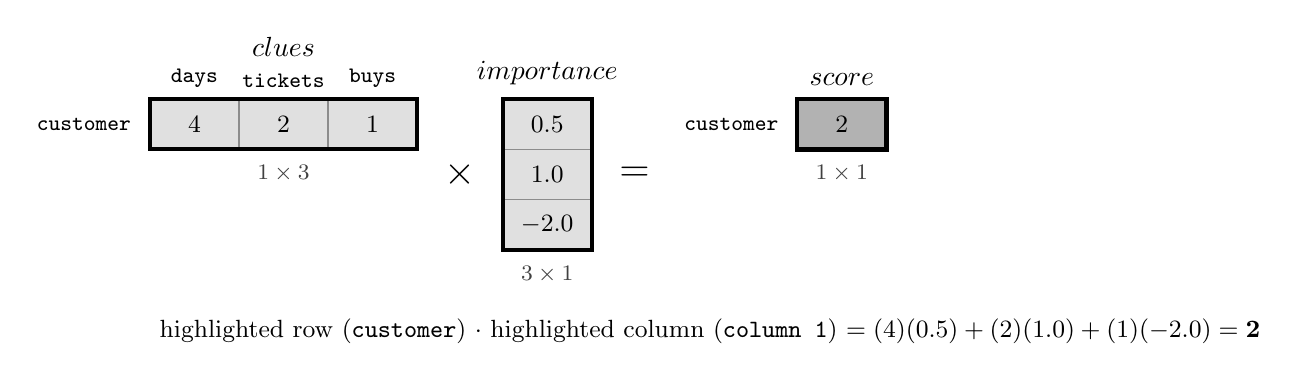
\begin{tikzpicture}[x=1.45cm]
\draw[black!45, fill=black!12] (0.000,0.000) rectangle (0.780,-0.640);
\node[font=\small, text=black] at (0.390,-0.320) {$4$};
\draw[black!45, fill=black!12] (0.780,0.000) rectangle (1.560,-0.640);
\node[font=\small, text=black] at (1.170,-0.320) {$2$};
\draw[black!45, fill=black!12] (1.560,0.000) rectangle (2.340,-0.640);
\node[font=\small, text=black] at (1.950,-0.320) {$1$};
\draw[line width=1.4pt] (0.000,0.000) rectangle (2.340,-0.640);
\draw[line width=0.9pt] (0.000,0.000) rectangle (2.340,-0.640);
\node[anchor=east, font=\footnotesize\ttfamily] at (-0.080,-0.320) {customer};
\node[anchor=south, font=\footnotesize\ttfamily] at (0.390,0.020) {days};
\node[anchor=south, font=\footnotesize\ttfamily] at (1.170,0.020) {tickets};
\node[anchor=south, font=\footnotesize\ttfamily] at (1.950,0.020) {buys};
\node[anchor=south, font=\normalsize] at (1.170,0.420) {$\text{clues}$};
\node[anchor=north, font=\footnotesize, text=black!75] at (1.170,-0.720) {$1\times3$};
\draw[black!45, fill=black!12] (3.090,0.000) rectangle (3.870,-0.640);
\node[font=\small, text=black] at (3.480,-0.320) {$0.5$};
\draw[black!45, fill=black!12] (3.090,-0.640) rectangle (3.870,-1.279);
\node[font=\small, text=black] at (3.480,-0.959) {$1.0$};
\draw[black!45, fill=black!12] (3.090,-1.279) rectangle (3.870,-1.919);
\node[font=\small, text=black] at (3.480,-1.599) {$-2.0$};
\draw[line width=1.4pt] (3.090,0.000) rectangle (3.870,-1.919);
\draw[line width=0.9pt] (3.090,0.000) rectangle (3.870,-1.919);
\node[anchor=south, font=\normalsize] at (3.480,0.050) {$\text{importance}$};
\node[anchor=north, font=\footnotesize, text=black!75] at (3.480,-1.999) {$3\times1$};
\draw[black!45, fill=black!30] (5.670,0.000) rectangle (6.450,-0.640);
\node[font=\small, text=black] at (6.060,-0.320) {$2$};
\draw[line width=1.6pt] (5.670,0.000) rectangle (6.450,-0.640);
\draw[line width=0.9pt] (5.670,0.000) rectangle (6.450,-0.640);
\node[anchor=east, font=\footnotesize\ttfamily] at (5.590,-0.320) {customer};
\node[anchor=south, font=\normalsize] at (6.060,0.050) {$\text{score}$};
\node[anchor=north, font=\footnotesize, text=black!75] at (6.060,-0.720) {$1\times1$};
\node[font=\Large] at (2.715,-0.959) {$\times$};
\node[font=\Large] at (4.245,-0.959) {$=$};
\node[anchor=north west, font=\small, align=left] at (0,-2.669) {highlighted row (\texttt{customer}) $\cdot$ highlighted column (\texttt{column 1}) $= (4)(0.5) + (2)(1.0) + (1)(-2.0) = \mathbf{2}$};
\end{tikzpicture}
